\documentclass[12pt]{article}

%\textwidth=20cm
%\textheight=16cm
%\setlength{\oddsidemargin}{-1cm}
\pdfoutput=1
\setlength\parindent{0pt}

\usepackage{jheppub}
\usepackage{graphicx,epsfig,amsmath,amssymb,mathtools}
%\usepackage{multirow,bigdelim,lscape}
%\usepackage{caption}
\usepackage{subcaption}
\usepackage{xspace}
%\usepackage{listings}
%\lstset{basicstyle=\ttfamily}
%% 
%\usepackage{titlesec}
\graphicspath{{plots/}}


%%% Macros
\newcommand\TwoFigBottom{-2}
%
\newcommand{\eqn}[1]{Eq.~(\ref{#1})}
\newcommand{\ab}{\ensuremath{\alpha_0}}
\newcommand{\als}{\ensuremath{\alpha_s}}
\newcommand{\gb}{\ensuremath{g_0}}
\newcommand{\gs}{\ensuremath{g}}
\newcommand{\mub}{\ensuremath{\mu_0}}
\newcommand{\mur}{\ensuremath{\mu_R}}
\newcommand{\amp}{\ensuremath{\mathcal{A}}}
\newcommand{\se}{\ensuremath{S_\epsilon}}
\newcommand{\msbar}{\ensuremath{\overline{\mathrm{MS}}}}
\newcommand{\gghh}{\ensuremath{{gg \rightarrow HH}}}
\newcommand{\gghhg}{\ensuremath{{gg \rightarrow HH + g}}}
\newcommand{\gqhhq}{\ensuremath{{gq \rightarrow HH + q}}}
\newcommand{\gqhhqb}{\ensuremath{{g\bar{q} \rightarrow HH + \bar{q}}}}
\newcommand{\qqhhg}{\ensuremath{{q\bar{q} \rightarrow HH + g}}}

\def\as{\frac{\alpha_s}{2\pi}}
\def\asm{\frac{\alpha_s^-}{2\pi}}
\def\ll{\log(M^2/\mu^2)}
\def\eps{\epsilon}
\def\shat{\hat{s}}
\def\that{\hat{t}}
\def\be{\begin{equation}}
\def\ee{\end{equation}}
\def\bea{\begin{eqnarray}}
\def\eea{\end{eqnarray}}
\def\nn{\nonumber}
\def\Ga{\Gamma}
\def\ket#1{|{#1}\rangle}
\def\bra#1{\langle{#1}|}
\def\braket#1#2{\langle #1 |#2 \rangle}
\def\bom#1{{\mbox{\boldmath $\mathrm{#1}$}}}

\newcommand{\powheg}{{\tt POWHEG}}
\newcommand{\powhegbox}{{\tt POWHEG-BOX}}
\newcommand{\secdec}{\textsc{SecDec}}
\newcommand{\gosam}{\textsc{GoSam}{}}
\newcommand{\form}{{\tt FORM}}
\newcommand{\golem}{{\tt Golem95}}
\newcommand{\ninja}{{\tt Ninja}}
\newcommand{\avholo}{{\tt OneLOop}}
\newcommand{\pythia}{{\tt Pythia\,8}\xspace}
\newcommand{\pyth}{{\tt Pythia}\xspace}
\newcommand{\pythiaold}{{\tt Pythia\,6}\xspace}
\newcommand{\herwig}{{\tt Herwig\,7.1}\xspace}
\newcommand{\herw}{{\tt Herwig}\xspace}
\newcommand{\hdamp}{{\tt hdamp}}
\newcommand{\idel}{i\,\delta}
\newcommand{\rd}{{\mathrm{d}}}
\newcommand{\loopint}[1]{\int \!\!\! \frac{d^D #1}{\left(2\pi\right)^D}\!}
\newcommand{\dd}[1]{\mathrm{d}#1\,}
\newcommand{\deltafun}{\,\delta}
\newcommand{\thetafun}{\,\theta}
\newcommand{\GeV}{\ensuremath{\mathrm{GeV}}}
\newcommand{\TeV}{\ensuremath{\mathrm{TeV}}}
\DeclareMathOperator{\re}{Re}
\DeclareMathOperator{\im}{Im}

\newcommand{\cg}{c_{ggh}}
\newcommand{\cgg}{c_{gghh}}
\newcommand{\ctt}{c_{tt}}
\newcommand{\ct}{c_{t}}
\newcommand{\cb}{c_{b}}
%$\newcommand{\chhh}{c_{hhh}}
\newcommand{\chhh}{\kappa_{\lambda}}
\newcommand{\mhh}{m_{hh}}
\newcommand{\pth}{p_{T,h}}
\newcommand{\pthh}{p_T^{hh}}
\newcommand{\ftapprox}{FT$_{\mathrm{approx}}$}




\def\ait#1{{\color{red}[~\textbf{#1}~]}}


%%%%%%%%%%%%%%%%%%%%%%%%%%%%%%%%%%%%%%%%%%%%%%%%%%%%%%%%%%%%%%%%%%%%%%%%%%%%%%%

%\begin{frontmatter}

\title{Probing the trilinear Higgs boson coupling in di-Higgs production at NLO QCD including parton shower effects}

\author[a]{G.~Heinrich,}
\author[b]{S.~Jones,}
\author[c]{M.~Kerner,}
\author[a]{G.~Luisoni,}
\author[a]{L.~Scyboz}

 
\affiliation[a]{Max Planck Institute for Physics, F\"ohringer Ring 6,  80805 M\"unchen, Germany}
\affiliation[b]{Theoretical Physics Department, CERN, Geneva, Switzerland}
\affiliation[c]{Physik-Institut, Universit{\"a}t Z{\"u}rich, Winterthurerstrasse 190, 8057 Z{\"u}rich, Switzerland}

\emailAdd{gudrun@mpp.mpg.de}
\emailAdd{s.jones@cern.ch}
\emailAdd{mkerner@physik.uzh.ch}
\emailAdd{luisonig@gmail.com}
\emailAdd{scyboz@mpp.mpg.de}


\preprint{{\small  CERN-TH-2019-x, MPP-2019-xx, ZU-TH yy/19, }}

\abstract{
 We present  NLO QCD results for Higgs boson pair 
  production with variations of the trilinear Higgs boson coupling, and with full top quark mass dependence.
  We provide differential results at 14\,TeV  and discuss
  the implications of anomalous trilinear couplings as well as differences between \pyth and \herw parton showers in combination with \powheg.
 The implementation of the NLO QCD calculation in the {\tt POWHEG-BOX-V2}
  Monte Carlo framework is publicly available.
}
 

\keywords{Higgs phenomenology, NLO QCD, BSM, future colliders}
%\end{frontmatter}


\begin{document}

\maketitle

\section{Introduction}

The Higgs potential is the least explored part of the Standard Model (SM) so far, and therefore measurements of the Higgs boson self-coupling(s) may offer surprises.
While the Higgs boson couplings to vector bosons and third generation fermions are increasingly well measured meanwile~\cite{Khachatryan:2016vau,ATLAS:2018doi,Sirunyan:2018koj}, constraints on the trilinear coupling $\lambda$ are weak due to the small cross section of Higgs boson pair production~\cite{Glover:1987nx,Dawson:1998py,Baglio:2012np,Frederix:2014hta,Borowka:2016ehy,Borowka:2016ypz,Baglio:2018lrj}.
Nonetheless, measurements of double Higgs production in gluon fusion, combining various decay channels,  have led to impressive experimental results already~\cite{Sirunyan:2018two,ATLAS-CONF-2018-043}, 
the most stringent constraints being $-5\leq \kappa_\lambda\leq 12.1$
 at 95\% confidence level~\cite{ATLAS-CONF-2018-043}.
Therefore, the determination of the trilinear coupling has entered a level of precision where the assumption that the full NLO QCD corrections do not vary much with $\kappa_\lambda$, which has been used in the experimental analysis so far, needs to be revised.
The variations of the K-factors with $\kappa_\lambda$ are mild in the $m_t\to \infty$ limit, where NLO~\cite{Grober:2015cwa,Grober:2017gut} and NNLO~\cite{deFlorian:2017qfk} corrections have been calculated within an effective Lagrangian framework.
However, it will be shown in this paper that the NLO K-factor varies by about 35\% as $\kappa_\lambda$ is varied between $-1$ and 5 once the full top quark mass dependence is taken into account. 

%Ref.~\cite{Buchalla:2018yce} is based on a non-linear Effective Field Theory which allows to focus on five anomalous couplings in the Higgs sector, $\chhh(=\kappa_\lambda), \ct,\ctt,\cg$ and $\cgg$, containing the full top quark mass dependence at NLO.

% Experimental constraints from current LHC data~\cite{Khachatryan:2016vau,Sirunyan:2018iwt,Aaboud:2018ftw} suggest that the trilinear Higgs boson coupling, relative to its Standard Model (SM) value, should be in the range $-8.2\leq \kappa_\lambda\leq 13.2$~\cite{Aaboud:2018ftw}, which still leaves quite some room for physics beyond the SM.
%While it is unlikely that New Physics alters just the Higgs boson self-couplings but leave the Higgs couplings to vector bosons and fermions unchanged, there is a plethora of consistent models where the deviations of the measured Higgs couplings from their SM values are so small that they have escaped detection so far. 
%while $|\kappa_\lambda|$ still can be large.
%Therefore it is very important to have precise predictions for observables which allow to measure the Higgs boson couplings. 
%This is particularly true for the trilinear Higgs self-coupling $\lambda$.

\medskip

In this work we study the dependence of total cross sections and differential distributions on the trilinear Higgs boson coupling, assuming that the deviations in the other couplings are at the (sub-)percent level.
The study is based on results at NLO QCD with full top quark mass dependence for Higgs boson pair production in gluon fusion described in Refs.~\cite{Borowka:2016ehy,Borowka:2016ypz}. 
While it is unlikely that New Physics alters just the Higgs boson self-couplings but leaves the Higgs couplings to vector bosons and fermions unchanged, there is a plethora of consistent models where the deviations of the measured Higgs couplings from their SM values are so small that they have escaped detection so far. 
As there is destructive interference in the squared amplitude between contributions containing $\lambda$ and those without the Higgs boson self-coupling (corresponding to triangle- and box diagrams at LO), 
%where the destructive interference is maximal at $\lambda\sim 2.4$, 
small changes in $\lambda$ modify the interference pattern and therefore can have a substantial effect on the cross sections.

To obtain a full-fledged NLO generator which also offers the possibility of parton showering, we implemented the calculation in the 
\powhegbox~\cite{Nason:2004rx,Frixione:2007vw,Alioli:2010xd}, building on the SM code presented in Ref.~\cite{Heinrich:2017kxx}.

The scale uncertainties at NLO are still at the 10\% level, while they are decreased to about 5\% when including the NNLO corrections
in the $m_t\to\infty$ limit~\cite{deFlorian:2013jea,Grigo:2015dia,deFlorian:2016uhr}. The calculation of Ref.~\cite{deFlorian:2016uhr} has been combined with results including the top quark mass dependence as far as available in Ref.~\cite{Grazzini:2018bsd}, and the latter has been supplemented by soft gluon resummation in Ref.~\cite{deFlorian:2018tah}. 
The uncertainties due to the chosen top mass scheme have been assessed in Ref.~\cite{Baglio:2018lrj}, where the full NLO corrections, including the possibility to switch between pole mass and $\overline{MS}$ mass, have been presented.

The dependence of the K-factors on the value for $\lambda$ (and other BSM couplings) is stronger than the $m_t\to\infty$ limit may suggest, as shown in Ref.~\cite{Buchalla:2018yce}. This is particularly true for differential K-factors, 
in combination with the $b\bar{b}$ decay channel of the Higgs boson, where in the boosted regime large-$p_T$ Higgs bosons are involved, which means that the top quark loops are resolved, such that the  $m_t\to\infty$ limit is clearly invalid.
The top quark mass corrections in the large $\mhh$ or $\pth$ regime being of the order of 20-30\% or higher, and increasing with larger centre-of-mass energy (e.g. $\sqrt{s}=27$ or 100\,TeV), these corrections clearly exceed the scale uncertainties and therefore have to be taken into account.

The purpose of this paper is twofold: Based on our differential results, we discuss how the deviations from the SM, resultig from non-SM $\lambda$ values, can be cornered based on the distributions for the Higgs boson pair invariant mass and Higgs boson transverse momentum distributions. 
In addition, we present the public code {\tt POWHEG-BOX-V2/ggHH}, where the user can choose the value of the trilinear coupling as an input parameter.
We also explain how variations of the top-Higgs Yukawa coupling can be performed with this code.
Further, we compare the fixed order results to results obtained after parton showering. In particular, we compare results from the \pythia~\cite{Sjostrand:2014zea} and \herwig~\cite{Bellm:2017bvx} parton showers and assess the parton-shower related uncertainties.

This paper is organised as follows. In Section~\ref{sec:calculation} we briefly describe the calculation and give instructions for the usage of the program within the \powhegbox. Section~\ref{sec:results} contains the discussion of our results, focusing in the second part on differences between results obtained with different parton showers, 
before we conclude in Section~\ref{sec:conclusions}.



\section{Overview of the calculation}
\label{sec:calculation}

The calculation builds on the one presented in Ref.~\cite{Heinrich:2017kxx} and therefore will be described only briefly here. 

The leading order amplitude in the full theory and  all the
amplitudes in the $m_t\to\infty$ limit were implemented analytically, whereas the
one-loop real radiation contribution and the two-loop virtual
amplitudes in the full SM rely on numerical or semi-numerical
codes.
The real radiation matrix elements in the full SM were implemented
using the interface~\cite{Luisoni:2013cuh}
between \gosam~\cite{Cullen:2011ac,Cullen:2014yla} and
the \powhegbox~\cite{Nason:2004rx,Frixione:2007vw,Alioli:2010xd}, modified
accordingly to compute the real corrections instead of the virtual ones. 
%The one-loop real amplitudes we generated with the version 2.0 of \gosam{}~\cite{Cullen:2014yla}, 
%which uses {\tt Qgraf}~\cite{Nogueira:1991ex}, \form~\cite{Kuipers:2012rf} and
%{\tt spinney}~\cite{Cullen:2010jv} for the generation of the Feynman
%diagrams, and offers a choice from {\tt Samurai}~\cite{Mastrolia:2010nb,vanDeurzen:2013pja}, {\tt golem95C}~\cite{Binoth:2008uq,Cullen:2011kv,Guillet:2013msa}
%and \ninja{}~\cite{Peraro:2014cba} for the
%reduction.  At run time the amplitudes were computed using
%\ninja{}~\cite{Peraro:2014cba} and \avholo{}~\cite{vanHameren:2010cp}
%for the evaluation of the scalar one-loop integrals.

For the virtual two-loop amplitudes, we have used the results of the
calculation presented in Refs.~\cite{Borowka:2016ehy,Borowka:2016ypz},
which used also {\sc Reduze}\,2~\cite{vonManteuffel:2012np} and {\sc
 SecDec}\,3~\cite{Borowka:2015mxa}.

The values for the Higgs boson and top quark masses have been set to
$m_h=125$\,GeV and $m_t=173$\,GeV, such that the two-loop amplitudes
only depend on two independent variables, the parton-level Mandelstam invariants
$\hat{s}$ and $\hat{t}$.  We have constructed a grid in these
variables together with an interpolation framework, such that an
external program can call the virtual two-loop amplitude at any phase space
point without having to do costly two-loop integrations.
We used the same setup for the grid as described in Ref.~\cite{Heinrich:2017kxx} and extended it in the following way:
We can write the squared matrix element as a polynomial of degree two in $\lambda$, 
\begin{align}
M_\lambda& \equiv |{\cal M}_\lambda|^2=A+B\,\lambda + C\,\lambda^2\;. \label{eq-amplambdadep}
\end{align}
Therefore it is sufficient to know the amplitude at three different values of $\lambda$ in order to reconstruct the full $\lambda$-dependence. 
Choosing $\lambda=-1,0,1$ we obtain
\begin{align}
A&=M_0\;,\; B=(M_1-M_{-1})/2\;,\; C=(M_1+M_{-1})/2-M_0\;.
\end{align}
In practice we used the representation 
\begin{align}
M_\lambda &=M_0\,(1-\lambda^2)+\frac{M_1}{2}\,(\lambda+\lambda^2) + \frac{M_{-1}}{2}\,(-\lambda+\lambda^2)\;
\end{align}
in order to get a more straightforward uncertainty estimate.

In fact, to any order in QCD, neglecting diagrams with quartic Higgs couplings, we can separate the matrix element into a 
piece that depends only on the top quark Yukawa coupling $y_t$ (``box diagrams'') and a 
piece that depends on the Higgs boson trilinear self-coupling $\lambda$ (``triangle diagrams''):
\begin{align}
{\cal M} = y_t^2 {\cal M}_B + y_t \lambda {\cal M}_T.
\end{align}
The squared amplitude at each order can then be written as
\begin{align}
|{\cal M}|^2 = y_t^4 \left[ {\cal M}_B {\cal M}_B^* + \frac{\lambda}{y_t} ({\cal M}_B {\cal M}_T^* + {\cal M}_T {\cal M}_B^* ) +  \frac{\lambda^2}{y_t^2} {\cal M}_T {\cal M}_T^*  \right].
\end{align}
The above parametrisation makes it clear that the dependence of the cross section on
both the Yukawa coupling and the Higgs boson self-coupling can be reconstructed
from only the 3 terms present in Eq.~(\ref{eq-amplambdadep}).

In order to allow for comparisons and cross checks, we implemented
both the $m_t\to\infty$ limit as well as the full SM amplitudes at
NLO. This allows to run the code in four different modes by changing
the flag {\tt mtdep} in the \powhegbox{} run card. The possible
choices are the following:
\begin{description}
 \item[{\tt mtdep=0}:]{computation using basic HEFT ($m_t\to\infty$ limit),}
 \item[{\tt mtdep=1}:]{computation using Born-improved HEFT ($m_t\to\infty$ limit rescaled with LO(full)/LO($m_t\to\infty$)),}
 \item[{\tt mtdep=2}:]{computation in the approximation \ftapprox (full
   mass dependence in the Born and in the real radiation, Born-improved HEFT
   for the virtual part),}
 \item[{\tt mtdep=3}:]{computation in the full SM.}
\end{description}

\vspace*{1cm}

When {\tt mtdep=3} is selected, the result of the virtual matrix element is based on a grid of pre-sampled phase-space points as described above. The phase-space points present in the grid are distributed such that they optimally sample the SM Born matrix element. The same grid of points is used regardless of the value of $\lambda$ selected. Due to the finite number of points present in the grid, there is an associated statistical uncertainty which amounts to $0.1\%$ on the total cross section at $14\ \TeV$ for $\lambda=\lambda_\mathrm{SM}$. However, for $\lambda \neq \lambda_\mathrm{SM}$ the virtual matrix element can differ significantly in shape from the SM prediction, as is apparent from examining the $\mhh$ and $\pth$ distributions for different values of the Higgs boson self coupling. The uncertainty associated with the use of the grid is therefore larger for non-SM values of $\lambda$. The uncertainty increases as $\lambda$ is decreased below the SM value reaching $0.6\%$ on the total cross section at $14\ \TeV$ for $\chhh = -1$. Increasing $\lambda$ above the SM value, we obtain an uncertainty of $3\%$ on the total cross section at $14\ \TeV$ for $\chhh = 3$ and  $\chhh = 5$. Furthermore, for differential distributions the total uncertainty is not distributed uniformly in each bin but instead increases when the shape of the matrix element most differs from the SM prediction. Focusing on the invariant mass distribution, amongst the values of the Higgs boson self-coupling considered here, the largest uncertainty is obtained for the smallest values of $\mhh$ and $\chhh=3$. The uncertainty reaches $6\%$ for the lowest bin when a $40\ \GeV$ bin width is used.


\section{Total and differential cross sections at non-SM trilinear couplings}
\label{sec:results}


The results were obtained using the
PDF4LHC15{\tt\_}nlo{\tt\_}30{\tt\_}pdfas~\cite{Butterworth:2015oua,CT14,MMHT14,NNPDF}
parton distribution functions interfaced to our code via
LHAPDF~\cite{Buckley:2014ana}, along with the corresponding value for
$\alpha_s$.  The masses of the Higgs boson and the top quark have been
fixed, as in the virtual amplitude, to $m_h=125$\,GeV, $m_t=173$\,GeV. Their widths have been set to zero.   
Jets are clustered with the
anti-$k_T$ algorithm~\cite{Cacciari:2008gp} as implemented in the
{\tt fastjet} package~\cite{Cacciari:2005hq, Cacciari:2011ma}, with jet
radius $R=0.4$ and a minimum transverse momentum 
$p_{T,\mathrm{min}}^{\rm{jet}}=20$\,GeV.  The scale uncertainties are
estimated by varying the factorisation/renormalisation scales
$\mu_{F}, \mu_{R}$. The scale variation bands 
represent scale variations around the central scale $\mu_0 =\mhh/2$, with
$\mu_{R} = \mu_{F}=c\,\mu_0$, where $c \in \{0.5,1,2\}$.
For the case $\lambda=\lambda_{\mathrm{SM}}$ we checked that the bands
obtained from these variations coincide with the bands resulting from
7-point scale variations. The PDF uncertainties have been studied in
\cite{deFlorian:2016spz} and found to be in general considerably smaller than the scale uncertainties.

\subsection{Total cross sections at different values of the trilinear coupling}

In Table \ref{tab:sigmatot} we list total cross sections at 13, 14 and 27\,TeV for various values of the trilinear Higgs coupling $\lambda$. 
\begin{table}[htb]
\begin{center}
%\setlength{\extrarowheight}{3.0pt}
\begin{tabular}{| c | c | c |c|c|}
%\Xhline{2\arrayrulewidth}
\hline
&&&&\\
$\lambda_{\mathrm{BSM}}/\lambda_{\mathrm{SM}}$ & $\sigma_{\rm{NLO}}@13 \mathrm{TeV}$\,[fb]& $\sigma_{\rm{NLO}}@14 \mathrm{TeV}$\,[fb] & $\sigma_{\rm{NLO}}@27 \mathrm{TeV}$\,[fb] &K-factor@14TeV\\
&&&&\\
\hline
-1& 116.71$^{+16.4\%}_{-14.3\%}$  & 136.91$^{+16.4\%}_{-13.9\%}$& 504.9 & 1.86 \\
\hline
0& 62.51$^{+15.8\%}_{-13.7\%}$ & 73.64$^{+15.4\%}_{-13.4\%}$& 275.29& 1.79  \\
\hline 
1& 27.84$^{+11.6\%}_{-12.9\%}$ & 32.88$^{+13.5\%}_{-12.5\%}$&127.7$^{+11.5\%}_{-10.4\%}$ &1.66\\
\hline
2 & 12.42$^{+13.1\%}_{-12.0\%}$ & 14.75$^{+12.0\%}_{-11.8\%}$ &  59.10 & 1.56 \\
\hline
2.4& 11.65$^{+13.9\%}_{-12.7\%}$ & 13.79$^{+13.5\%}_{-12.5\%}$& 53.67 & 1.65 \\
\hline
3& 16.28$^{+16.2\%}_{-15.3\%}$ & 19.07$^{+17.1\%}_{-14.1\%}$ & 69.84 & 1.90 \\
\hline 
5& 81.74$^{+20.0\%}_{-15.6\%}$  & 95.22$^{+19.7\%}_{-11.5\%}$& 330.61 & 2.14 \\
\hline 
\end{tabular}
\end{center}
\caption{Total cross sections for Higgs boson pair production at full NLO QCD. The given uncertainties are scale uncertainties. 
\label{tab:sigmatot}}
\end{table}
Table~\ref{tab:sigmatot} also shows that the K-factors vary substantially as functions of the trilinear coupling.
This fact is illustrated in Fig.~\ref{fig:Kfacvariation}, showing that the K-factor takes values between 1.56 and 2.14
if the trilinear coupling is varied between $-5\leq \chhh\leq 12$.

\begin{figure}[htb]
  \centering
    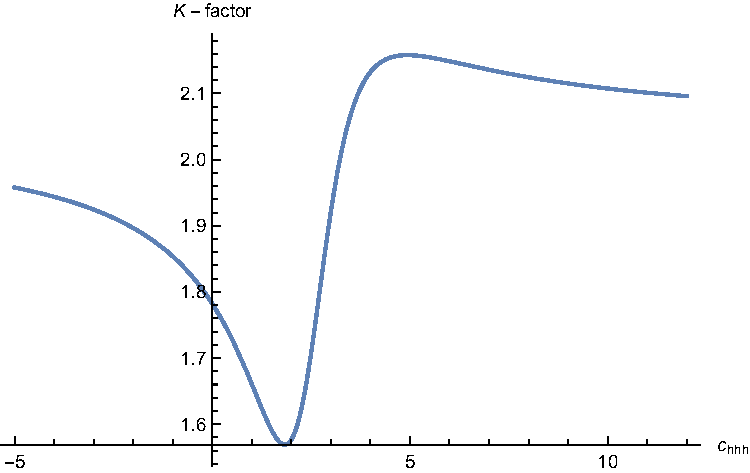
\includegraphics[width=0.45\textwidth]{plots/Kfac_varlambda.pdf}
%  \includegraphics[width=\textwidth]{plots/}
%    \caption{\label{fig:lambda_large_27}}
\caption{Variation of the NLO K-factor with the trilinear coupling at $\sqrt{s}=14$\,TeV.}
\label{fig:Kfacvariation}
\end{figure}


\subsection{Differential cross sections}

In Fig.~\ref{fig:lambdavar14TeV} we show the $\mhh$ distribution for various values of $\chhh=\lambda_{\mathrm{BSM}}/\lambda_{\mathrm{SM}}$. 
The ratio plots show the ratio to the result with $\lambda_{\mathrm{SM}}$. 
A characteristic dip develops in the $\mhh$ distribution around $\chhh=2.4$, which is the value of maximal destructive interference between diagrams containing the trilinear coupling (triangle-type contributions) and ``background" diagrams (box-type contributions).
Therefore we provide results for a denser spacing of $\chhh$ values around this point.

\begin{figure}[htb]
 \begin{subfigure}[t]{0.495\textwidth}
\includegraphics[width=\textwidth]{plots/{NLO_cHHH_1_2_2.4_0_mHH-paper}.pdf}
%    \vspace{\TwoFigBottom em}
\caption{\label{fig:lambda_small}}
\end{subfigure}
\hfill
\begin{subfigure}[t]{0.495\textwidth}
    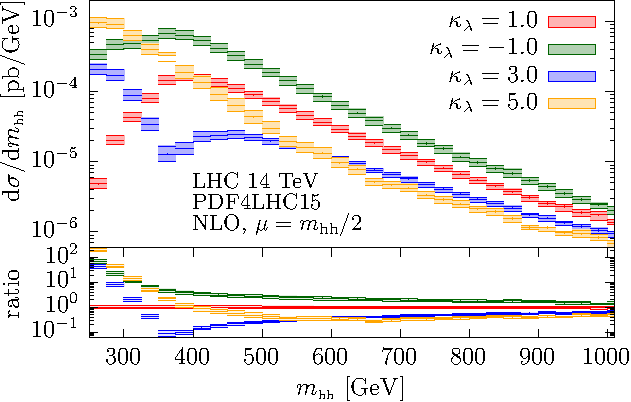
\includegraphics[width=\textwidth]{plots/NLO_cHHH_1_-1_3_5_mHH-paper.pdf}
\caption{\label{fig:lambda_large}}
\end{subfigure}
\caption{Higgs boson pair invariant mass distributions for various
  values of $\chhh$  at $\sqrt{s}=14$\,TeV. The uncertainty bands are from
  scale variations as described in the text.}
\label{fig:lambdavar14TeV}
\end{figure}

\begin{figure}[htb]
 \begin{subfigure}[t]{0.495\textwidth}
\includegraphics[width=\textwidth]{plots/{NLO_cHHH_1_2_2.4_0_ptH-a}.pdf}
\caption{\label{fig:lambda_small_pTH}}
\end{subfigure}
\hfill
\begin{subfigure}[t]{0.495\textwidth}
    \includegraphics[width=\textwidth]{plots/{NLO_cHHH_1_-1_3_5_ptH-a}.pdf}
\caption{\label{fig:lambda_large_pTH}}
\end{subfigure}
\caption{Higgs boson transverse momentum distributions for various values of $\chhh$  at $\sqrt{s}=14$\,TeV.
\label{fig:lambdavar14TeV_pTH}}
\end{figure}
In Fig.~\ref{fig:lambdavar14TeV_pTH} we show the transverse momentum
distributions $p_T^h$ of one (any) Higgs boson for different $\chhh$
values. The dip for $\chhh\sim 2.4$ is still present, however much
less pronounced than in the $\mhh$ distribution.

\begin{figure}[htb]
 \begin{subfigure}[t]{0.495\textwidth}
\includegraphics[width=\textwidth]{plots/{NLO_CPP_yt_0.8_1.2_mHH}.pdf}
\caption{\label{fig:ytvar_mhh}}
\end{subfigure}
\hfill
\begin{subfigure}[t]{0.495\textwidth}
\includegraphics[width=\textwidth]{plots/{NLO_CPP_yt_0.8_1.2_pTH-a}.pdf}
\caption{\label{fig:ytvar_pth}}
\end{subfigure}
\caption{Higgs boson pair invariant mass distributions, and distributions of the transverse momentum of one (any) Higgs boson for non-SM values of the top quark Yukawa coupling $y_t$  at $\sqrt{s}=14$\,TeV, including scale uncertainties.
\label{fig:ytvar}}
\end{figure}

Fig.~\ref{fig:ytvar} demonstrates the effect of variations of the top quark Yukawa coupling $y_t$ on the $\mhh$ and $\pth$ distributions, where $\chhh$ is fixed to the SM value.
Using eq.~(\ref{eq:yt}), it is apparent that $y_t$ variations can be obtained from appropriate $\chhh$ variations with the same code.
For example, $\sigma(y_t=1.2,\chhh=1)=(1.2)^4\,\sigma(y_t=1,\chhh=1/1.2)$.

\subsection{Discussion of parton shower related uncertainties} 
 
In this section we show distributions for NLO results matched to a
parton shower, focusing mostly on the transverse momentum of the Higgs
boson pair. For this distribution 
NLO is the first non-trivial order, and therefore it is particularly
sensitive to differences in the treatment of radiation by the
parton shower.
We compare the \pythia~\cite{Sjostrand:2014zea} and \herwig~\cite{Bellm:2017bvx} parton showers, 
applied directly to the \powheg{} Les Houches events (LHE).
In the \herw case, we also compare the default shower (the angular-ordered $\tilde{q}$-shower) 
with the dipole shower.
In addition, we assess the uncertainties stemming from the matching and show results where the 
\herw shower scale parameter {\tt HardScale} is varied. For all shower algorithms considered, the default 
tune of the corresponding version is used. Multiple-parton interactions (MPI) and hadronisation 
are switched off. The \hdamp{} parameter in \powheg{} is set to $\hdamp=250$\,GeV.

\begin{figure}[htb]
 \begin{subfigure}[t]{0.495\textwidth}
\includegraphics[width=\textwidth]{plots/{NLO_PP8_PH7_PH7D_cHHH_1_ptH-a}.pdf}
 \caption{\label{fig:lambda_pTh}}
\end{subfigure}
\hfill
\begin{subfigure}[t]{0.495\textwidth}
    \includegraphics[width=\textwidth]{plots/{NLO_PP8_PH7_PH7D_cHHH_1_dRHH}.pdf}
\caption{\label{fig:lambda_dRHH}}
\end{subfigure}
\caption{The transverse momentum of one (any) Higgs boson and the $R$-separation between 
the two Higgs bosons are shown for the fixed-order NLO calculation and three shower setups, in 
the $\chhh=1$ case.
\label{fig:lambdavar14TeV_pTH_dRHH_showers}}
\end{figure}

In general, observables that are inclusive in the additional radiation, like the 
transverse momentum of one (any) Higgs boson, $p_T^h$, show little sensitivity to the details of 
the parton showering, as can be seen from Fig.~\ref{fig:lambda_pTh}, showing the fixed-order NLO prediction, 
as well as  the \pythia (PP8) and both \herwig showers (angular-ordered PH7-$\tilde{q}$, 
and PH7-dipole). In contrast, Fig.~\ref{fig:lambda_dRHH} 
displays the distribution of the distance $\Delta
R^{\mathrm{hh}}=\sqrt{(\eta_1-\eta_2)^2+(\Phi_1-\Phi_2)^2}$ between the two Higgs 
bosons. There, the Sudakov exponent and the parton shower effectively resum the fixed-order 
prediction in the region where the two Higgs bosons are close to a back-to-back configuration, 
and the parton shower increases the fixed-order real radiation contribution in the region $\Delta R^{\mathrm{hh}}<\pi$.

\begin{figure}[htb]
 \begin{subfigure}[t]{0.495\textwidth}
\includegraphics[width=\textwidth]{plots/{NLO_PP8_PH7_PH7D_cHHH_1_ptHH}.pdf}
 \caption{\label{fig:lambda_ptHH_cHHH1}}
\end{subfigure}
\hfill
\begin{subfigure}[t]{0.495\textwidth}
    \includegraphics[width=\textwidth]{plots/{NLO_PP8_PH7_PH7D_cHHH_2.4_ptHH}.pdf}
\caption{\label{fig:lambda_ptHH_cHHH2.4}}
\end{subfigure}
\caption{Transverse momentum of the Higgs boson pair for the fixed-order NLO calculation 
and all three shower setups at 14\,TeV for (a) $\chhh=1$, (b) $\chhh=2.4$.
\label{fig:lambdavar14TeV_pTHH_showers}}
\end{figure}

In Figs.~\ref{fig:lambda_ptHH_cHHH1} and \ref{fig:lambda_ptHH_cHHH2.4}, the transverse 
momentum $\pthh$ of the Higgs boson pair system is shown for the fixed-order and parton-showered predictions, at $\chhh=1$ and $\chhh=2.4$. In all cases, the \pyth and \herw showers 
agree very well in the small-$\pthh$ range, but start to deviate already at $\pthh \sim 100$\,GeV. 
While both \herw showers give very similar results and reproduce the fixed-order calculation at high-$\pthh$, the 
\pyth shower produces much harder additional radiation and the ratio to the fixed-order result plateaus at $\sim 2.0$ over the remaining range. 
%A discussion of the surprisingly hard tail of the $\pthh$ distribution with \powheg+\pythia can be found in
%Refs.~\cite{Jones:2017giv,Bendavid:2018nar}, where the results are also
%compared to two different showers within {\sc Sherpa}~\cite{Gleisberg:2008ta,Schumann:2007mg,Hoche:2015sya} as well
%as with {\sc MG5\_aMC@NLO}~\cite{Alwall:2014hca,Hirschi:2015iia}.
We should mention that rather large differences between \pythia and
\herwig showers matched to \powheg{} also have been found studying top
quark pair production~\cite{Ravasio:2018lzi}. The origin of the large NLO parton shower matching uncertainties affecting certain observables in Higgs boson pair production have previously been studied in literature~\cite{Jones:2017giv}. For the SM result, the excess at large $\pthh$ produced when using \powheg{} with \pythia was found to be due to additional hard sub-leading jets generated purely by the shower~\cite{Bendavid:2018nar}.

With the \herw default shower, systematic uncertainties can be estimated by 
varying the maximal transverse momentum allowed for shower emissions,
by changing the so-called hard scale $\mu_Q$. We apply a factor $c_Q=\{0.5,\,2.0\}$ on the central hard shower scale, separately 
for all variations of the factorisation/renormalisation scales
$\mu_{R,F}$.
%, which is the standard use in the \herw setup. 
Fig.~\ref{fig:lambdavar14TeV_muQvar} shows the $\pthh$ and 
$\Delta R^{\mathrm{hh}}$ distributions as examples of the SM case, $\chhh=1$, and underlines 
their sensitivity to changes in the shower hard scale. Quantitatively, the hard scale variations 
inflate the sole factorisation/renormalisation scale uncertainties by a factor of two in 
the regions where the \herwig and \pythia showers were in disagreement (see Figs.~\ref{fig:lambda_dRHH} 
and \ref{fig:lambdavar14TeV_pTHH_showers}). If the envelope of all scale variations, including 
the hard shower scale, was to be taken as a theoretical systematic uncertainty, the resulting 
uncertainty would be of the order of 50\% in these bins. It would be enlightening to further study 
parton shower (and non-perturbative) effects, in the particular context of Higgs boson pair 
production at NLO, as well as for loop-induced colour singlet production in general, and try to reduce discrepancies among the different algorithms. 


\begin{figure}[htb]
 \begin{subfigure}[t]{0.495\textwidth}
\includegraphics[width=\textwidth]{plots/{PP8_PH7_PH7QUp_PH7QDown_cHHH_1_ptHH}.pdf}
 \caption{\label{fig:lambda_ptHH_muQvar}}
\end{subfigure}
\hfill
\begin{subfigure}[t]{0.495\textwidth}
    \includegraphics[width=\textwidth]{plots/{PP8_PH7_PH7QUp_PH7QDown_cHHH_1_dRHH}.pdf}
\caption{\label{fig:lambda_dRHH_muQvar}}\end{subfigure}
\caption{Higgs boson pair transverse momentum and $R$-separation for variations of the \herw $\tilde{q}$-shower hard scale.
\label{fig:lambdavar14TeV_muQvar}}
\end{figure}



\section{Conclusions}
\label{sec:conclusions}

We have presented results for Higgs boson pair production in gluon
fusion at full NLO for non-standard values of the trilinear Higgs
boson coupling $\lambda$. The total cross section is a quadratic
polynomial in $\lambda$, with a minimum around $\chhh\approx 2.4$,
which is present both at LO and NLO with full top quark mass
dependence, stemming from destructive interference of diagrams with
and without a trilinear Higgs coupling. 
The $\mhh$ distribution shows a dip around this minimum, which is to
less extent also visible in the transverse momentum distribution of
one of the Higgs bosons. 
We have assumed in our study that modifications of the Higgs couplings
to other particles are small and can be increasingly well constrained by
other processes. Nonetheless it should be kept in mind that a dip in
the $\mhh$ distribution could also originate from other effective
couplings, for example an effective $t\bar{t}HH$ coupling, while
$\chhh= 1$~\cite{Buchalla:2018yce}.

We have also combined our NLO QCD results with the \pythia and \herwig
parton showers, where in the \herwig case we employed both the default shower (the angular-ordered $\tilde{q}$-shower) and the dipole shower.
We observed that \ait{ToDo}.

The \powheg{} version of the code for Higgs boson pair production
including the possibility to vary the trilinear coupling 
and the top quark Yukawa coupling 
is publicly available in the \powhegbox{\tt-V2} package at the website
{\tt http://powhegbox.mib.infn.it}, in the
{\tt User-Processes-V2/ggHH/} directory.
.




\section*{Acknowledgements}
We would like to thank Gerhard Buchalla, Alejandro Celis, Matteo Capozi and Stephan Jahn for helpful discussions.
This research was supported in part by the COST Action CA16201 `Particleface' of the European Union.
We gratefully acknowledge resources provided by the Max Planck Computing and Data Facility (MPCDF).

%\clearpage

%%%%%%%%%%%%%%%%%%%%%%%%%%%%%%%%%%%%%%%%%%%%%%%%%%%%%%%%%%%%%% 
\bibliographystyle{JHEP}
 
\bibliography{refs_HH_lambda}

\end{document}
